\chapter{METODOLOGIA}

%Metodologia da bibliografia
\section{Metodologia usada no Levantamento Bibliográfico}


Para atingir os objetivos que orientam este estudo, os procedimentos metodológicos foram idealizados com base em programas educacionais que visam a promoção do empreendedorismo e comportamento empreendedor em cursos de graduação, em instituições de ensino públicas e particulares, como também Startups de natureza educacional.


A metodologia de pesquisa utilizada encontra-se esquematizada na Figura \ref{figura_referencial}. Buscando construir um levantamento bibliográfico sólido sobre os conteúdos pretendidos neste estudo, será realizada uma revisão sistemática utilizando como ferramenta o StArt \cite{lapes_start_2016}. A ferramenta StArt será desenvolvida para apoiar todo processo de Revisão Bibliográfica, por meio de uma árvore hierárquica, categorizando os artigos em proximidade e níveis de aderência às palavras-chave \cite{hernandes_avaliacao_2010}.


\begin{figure}[H]
\centering
\caption{\textbf{Planejamento da pesquisa e construção do referencial teórico}}
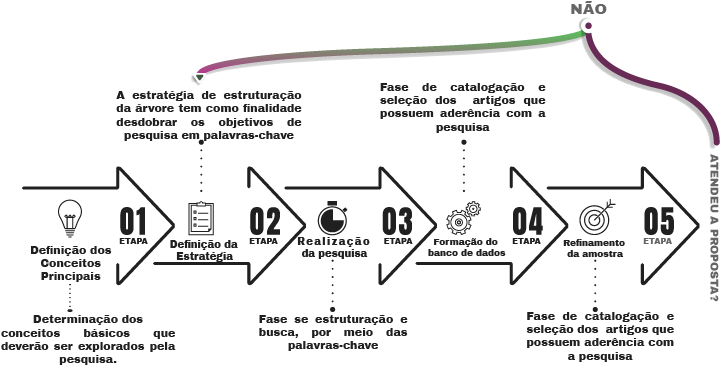
\includegraphics[scale=0.6]{Imagens/fases_pesquisa_bibliografica.png}
\fonte{O Autor adaptado de \cite{lapes_start_2016}}
\label{figura_referencial}
\end{figure}

\section{Metodologia usada no Levantamento dados sobre Transferências}

\subsection{Raspagem dos Dados}

Os dados sobre transferência de tecnologias desenvolvidas pelos órgãos públicos direcionadas ao setor agrícola foram selecionados a partir das publicações disponíveis no Diário Oficial da União DOU.

Para delimitar o ambiente de estudo, foram adotados como indicadores os termos “Transferência de tecnologia*” e “Agricultura/Agrícola”. 

Como linha temporal foram selecionados os comentários realizados de 2016 a 2020. Dos órgãos previamente pesquisados  constam: Universidades públicas, Centros de Pesquisa e Empresas públicas.

Objetivando preservar a identidade das empresas envolvidas neste estudo, estas serão descritas como: (UP) Universidade Pública, (CP) Centro de Pesquisa, (EP) Empresa pública.
Nesta fase do  estudo, será configurada, para a coleta automatizada, a raspagem web Octoparse (versão 7.1.2, Octopus Data Inc., Walnut, CA, USA). Este software é um sistema de Eletronic Data Scraping que permite a raspagem dos dados presentes em sites abertos. 

O software será programado para extrair os comentários sobre a percepção da estadia, desta forma, o processo de extração será realizado em cinco passos, a saber: acesso ao site de ofertas; paginação dos locais de hospedagem; loop de raspagem dos itens; extração dos dados e abertura de novas páginas. Este processo está descrito na Figura \ref{figura_raspagem}. Durante a coleta dos dados, as publicações que se mostraram em duplicidade foram suprimidos. 



\begin{figure}[H]
\centering
\caption{\textbf{Espaço de trabalho para raspagem de publicações no Diário Oficial da União sobre transferência de tecnologia agrícola.
}}
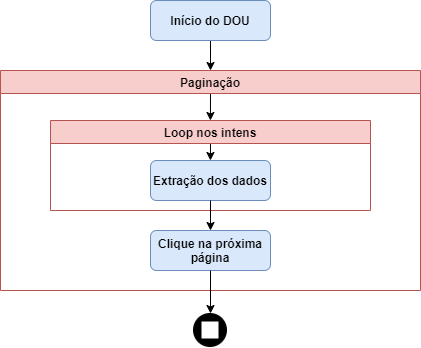
\includegraphics[scale=0.6]{Imagens/raspagem.png}
\fonte{Os Autores 2020.}
\label{figura_raspagem}
\end{figure}


\subsection{Análise quantitativa de dados textuais}

Após a seleção dos comentários diretamente relacionados ao tema proposto nesta pesquisa, foram realizadas lexicométricas e análises de discursos nos textos presentes com o auxílio do software IRaMuTeQ \cite{conde_lexicometria_2015,da_silva_cezar_panorama_2018}. Através da utilização de Unidades de Contexto Iniciais (UCIs) na construção do modelo para análise, será realizada uma prévia correção no conjunto de dados brutos mantendo as palavras analisáveis, os termos caracterizados como substantivos, adjetivos e verbos. As palavras que geralmente não são relevantes para uma análise, como preposições e advérbios, foram excluídas.

Ao se trabalhar com corpus textuais cada conjunto de texto deve compor uma UCI. Um conjunto de UCI é conhecido como corpus de análise, os quais o software segmenta em textos de aproximadamente três linhas, chamados de Segmento de Texto (ST) \cite{fernandes_avaliacao_2018}. Após a segmentação dos textos, o software realiza uma Categorização Hierárquica Descendente (CHD) dando origem a classes lexicais caracterizadas pelo vocabulário e a segmentos de textos que partilham o mesmo vocábulo.

A Classificação Hierárquica Descendente (CHD) consiste em um tipo de análise de conglomerado que categoriza as palavras obtidas em classes lexicais (eixos). A análise avalia a constância e os arranjos das palavras ativas que estão no corpus textual usando os dados das tabelas de contingência das palavras existentes \cite{carvalho_utilizacao_2020,mendes_mapping_2019}. Neste sentido, as diferentes classes resultantes representam o espaço de sentido das palavras narradas, surgindo, assim, elementos pertencentes aos temas observáveis da pesquisa \cite{gavasso_revisao_2016}. 

Por fim, é importante ressaltar que a avaliação da metodologia proposta neste estudo será mediada pela técnica desenvolvida por \citeonline{costa_construcao_2015} tendo como base a \textit{Assessment of Multiple Systematic Reviews} (AMSTAR).


\section{Desenvolvimento do Modelo conceitual para transferência de tecnologia agrícola}


Buscando categorizar as dimensões que serão utilizadas no modelo, optou-se os indicadores observados serão agrupados conforme as dimensões específicas para Transferência de Tecnologia. Para o desenvolvimentos dos parâmetros que compõem o modelo preliminar que será analisado pelo método Delphi, serão consideradas cinco dimensões: dimensão de sustentabilidade, perguntas-chave, indicador, descritor de inovação, nota e peso da tecnologia.

O método Delphi se baseia na aplicação estruturada do conhecimento e da experiência de especialistas da área pressupondo que, o julgamento em conjunto de determinado processo, quando organizado adequadamente, é melhor que a opinião de um só indivíduo.










